\documentclass[a4paper,12pt]{extreport}
\usepackage[a4paper, margin=1in]{geometry}
\usepackage{graphicx} % Required for inserting images
\usepackage{fontspec}
\usepackage{xunicode} % Enable line breaks for Thai text
\usepackage{xltxtra}
\usepackage{listings}
\usepackage{float}
\XeTeXlinebreaklocale "TH"
\XeTeXlinebreakskip = 0pt plus 2pt minus 1pt
\setmainfont[
  Path=Font/,
  BoldFont={THSarabunNew_Bold.ttf},
  ItalicFont={THSarabunNew_Italic.ttf},
  BoldItalicFont={THSarabunNew_BoldItalic.ttf},
]{THSarabunNew.ttf}
%% ---- Customizing LaTeX elements to Thai language ---- %%
\renewcommand{\chaptername}{บทที่}  % Change "Chapter" to "บทที่"
\renewcommand{\contentsname}{สารบัญ}  % Change "Contents" to "สารบัญ"
\renewcommand{\indexname}{ดัชนี}      % Change "Index" to "ดัชนี"
\renewcommand{\figurename}{ภาพที่}    % Change "Figure" to "ภาพที่"
\newcommand{\imgwidth}{0.6\linewidth}

\title{2110531 Data Science and Data Engineering Take-Home Midterm Exam\\Paper Classification Report (2024/1)}
\author{Krissada Sarawit\\6770215021}
\date{October 2024}
\begin{document}
\maketitle
\clearpage

\tableofcontents
\chapter{บทนำ}
\section{การกำหนดปัญหา}
ในโลกของการวิจัยทางวิชาการ
การแบ่งประเภทและการจำแนกวรรณกรรมมีบทบาทสำคัญในงานวรรณกรรม
เพื่อผู้อ่านสามารถค้นหาผลงานทางวิชาการที่เกี่ยวข้องได้นั้น 
จำเป็นต้องมีวิธีการแบ่งประเภทวรรณกรรมอย่างถูกต้องและแม่นยำ
ด้วยฐานข้อมูลอย่าง Scopus ที่มีบทความนับล้านบทความ
การแยกประเภทด้วยการการตีความโดยใช้มนุษย์จึงเป็นเรื่องที่ท้าทายและต้องใช้แรงงานอย่างมาก
วิธีแก้ปัญหาที่มีแนวโน้มที่ดีอย่างหนึ่งคือการจำแนกข้อความแบบหลายป้ายกำกับ หรือ Multi-label text classification

ปัญหา Multi-label text classification คือการจำแนกหมวดหมู่ของข้อความ โดยที่ข้อความหนึ่งสามารถเป็นไปได้หลากหลายหมวดหมู่ ปัญหาที่ได้รับในโจทย์จะเป็นการจำแนกบทความทางวิชาการในด้านวิศวกรรมศาสตร์ โดยแบ่งเป็น 18 สาขา ได้แก่ civil, environmental, biomedical, petroleum, metallurgical, mechanical, electrical, computer, optical, nano, chemical, materials, agricultural, education, industrial, safety, "mathematics and statistics", and material science.

\section{วัตถุประสงค์}
วัตถุประสงค์ของการทดลองในครั้งนี้คือการพัฒนาโมเดลการจำแนกข้อความหลายป้ายกำกับที่มีประสิทธิภาพซึ่งสามารถคาดการณ์หัวข้อต่าง ๆ ได้อย่างแม่นยำจากเอกสารบทคัดย่อและชื่องานวิจัย

เนื่องจากเอกสารแต่ละฉบับสามารถอยู่ในสาขาวิศวกรรมศาสตร์ที่แตกต่างกัน 18 สาขาแต่ละเอกสารสามารถอยู่ได้มากกว่า 1 สาขา โมเดลจัดหมวดหมู่จึงจำเป็นต้องเรียนรู้รูปแบบที่ซับซ้อนจากข้อความและกำหนดป้ายกำกับที่เหมาะสมซึ่งสะท้อนถึงลักษณะสหวิทยาการของเนื้อหา ซึ่งจะทำให้สามารถจัดหมวดหมู่วรรณกรรมทางวิศวกรรมศาสตร์ได้อย่างแม่นยำ ซึ่งจะช่วยให้นักวิจัยจัดระเบียบและค้นหาผลงานวิจัยที่เกี่ยวข้องในโดเมนวิศวกรรมศาสตร์ที่หลากหลายได้อย่างมีประสิทธิภาพ
\chapter{การสำรวจข้อมูล}
\section{Dataset Description}
Dataset สำหรับการ Train มีทั้งหมด 454 แถว 3 คอลลัมน์ ประกอบด้วย:
\begin{enumerate}
    \item Title ชื่อของงานวิจัย
    \item Abstract บทคัดย่อ
    \item Classes ป้ายกำกับสาขาของงานวิจัยนั้น
\end{enumerate}

ทำการโหลดไฟล์ train.json เข้า Pandas Dataframe
\begin{figure}[ht]
    \centering
    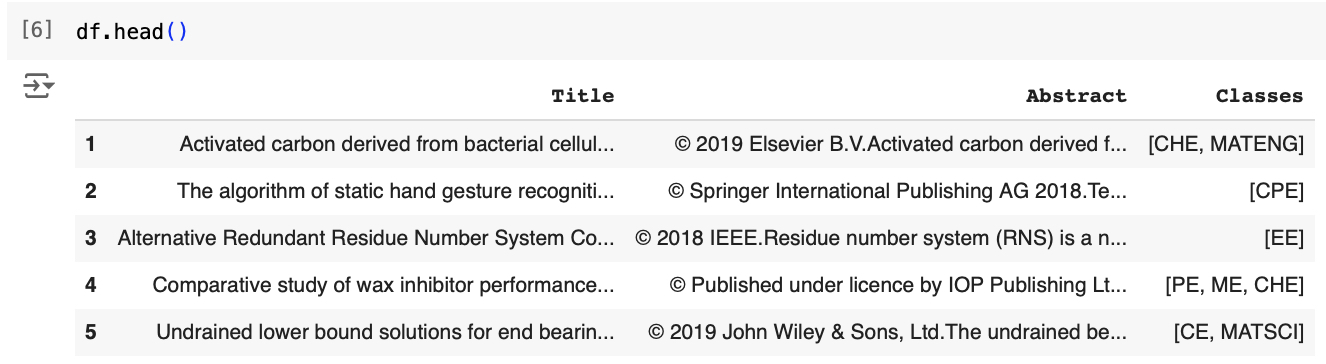
\includegraphics[width=\imgwidth]
    {images/dataframe_head.jpg}
    \caption{ตัวอย่าง Dataframe}
    \label{fig:dataframe_head}
\end{figure}
\clearpage


\begin{figure}
    \centering
    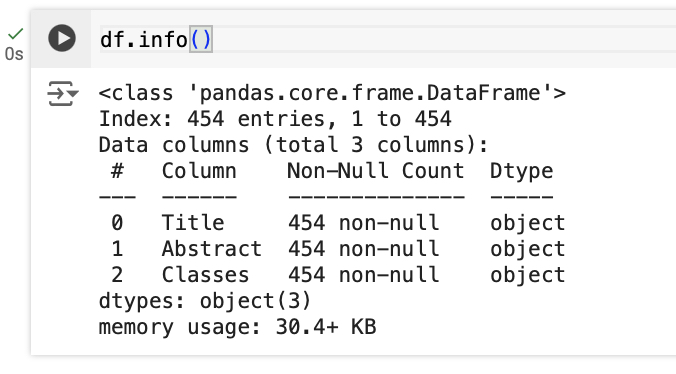
\includegraphics[width=\imgwidth]
    {images/dataframe_info.jpg}
    \caption{รายละเอียด Dataframe}
    \label{fig:dataframe_info}
\end{figure}
รายละเอียด Dataframe ประกอบด้วย 454 แถว และ 3 คอลลัมน์
\section{Data Statistics}
ดูการกระจายตัวของข้อมูลแต่ละคลาส พบว่าคลาสไม่่สมดุลกัน โดยที่คลาสที่มีมากที่สุดคือ CHE มีจำนวนมากถึง 177 แถวและคลาสที่มีจำนวนน้อยที่สุดคือ AGRI มีเพียง 20 แถว ดังนั้นจะต้องคำนวณ class weight เพื่อทำไปใช้ใน loss function
\begin{figure}[ht]
    \centering
    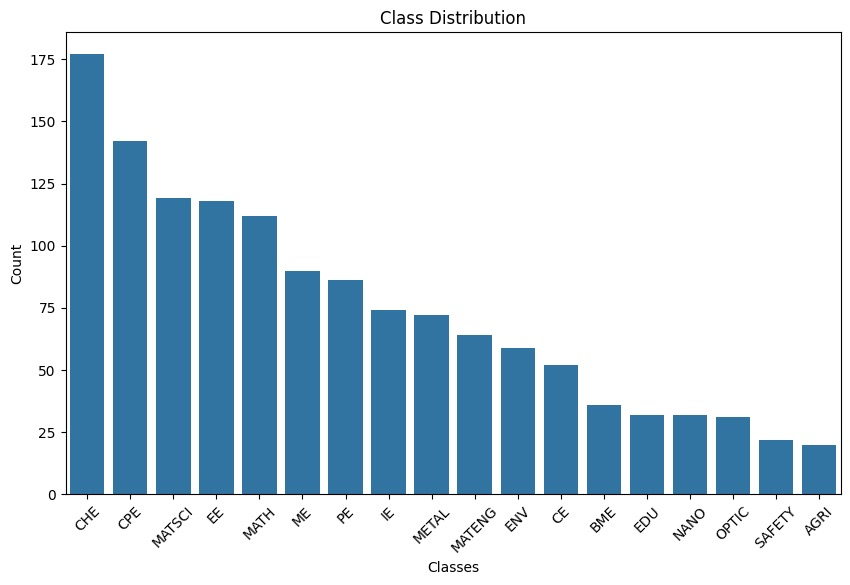
\includegraphics[width=\imgwidth]
    {images/class_distribution.jpg}
    \caption{การกระจายตัวของแต่ละ class}
    \label{fig:class_distribution}
\end{figure}


\section{Data Preprocessing}
การเตรียมข้อมูลประกอบด้วย แปลงให้ตัวอักษรเป็น lower case ลบตัวอักษรพิเศษ ลบเลข ลบช่องว่างที่ไม่จำเป็น และลดรูปคำให้เหลือเพียงคำฐานโดยใช้ spacy library \cite{spacy2}
\begin{figure}[ht]
    \centering
    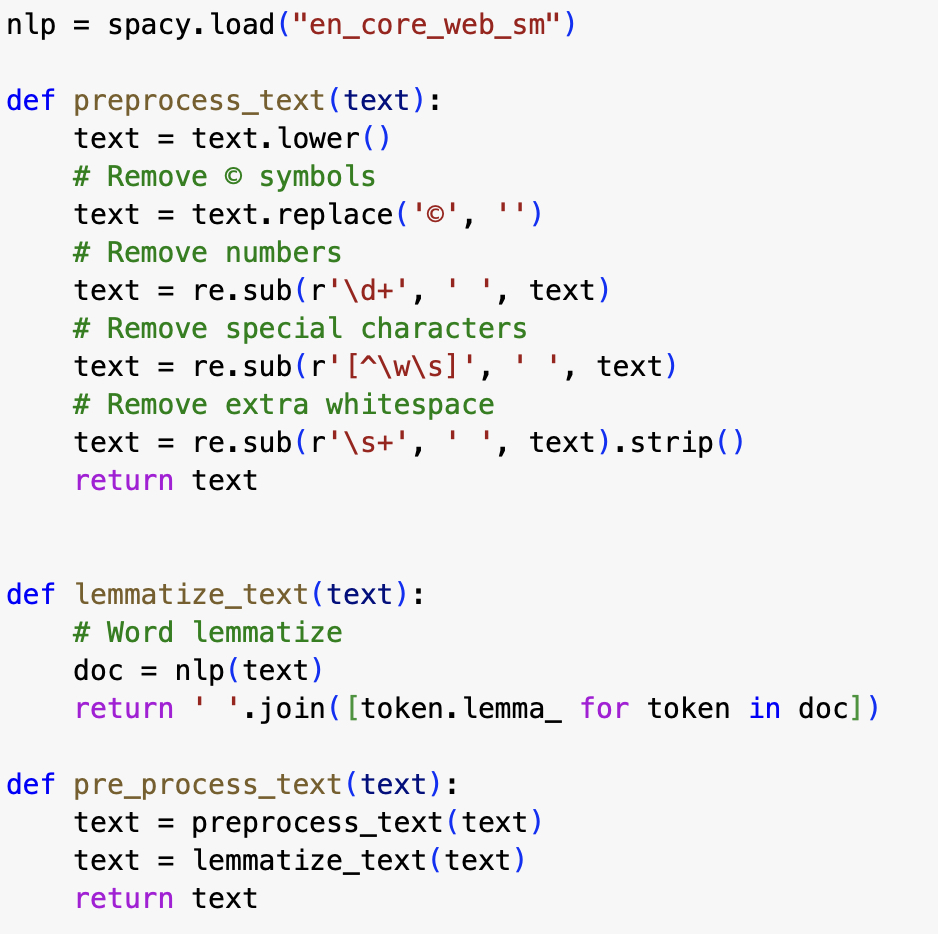
\includegraphics[width=\imgwidth]
    {images/preprocess.jpg}
    \caption{การ Preprocess Data}
    \label{fig:preprocess}
\end{figure}


หลังจากนั้นทำการแปลง Label ของข้อมูลให้เป็นรูปแบบ Binary ด้วย MultiLabelBinarizer จาก library scikit-learn \cite{pedregosa2011scikit}

\begin{figure}[ht]
    \centering
    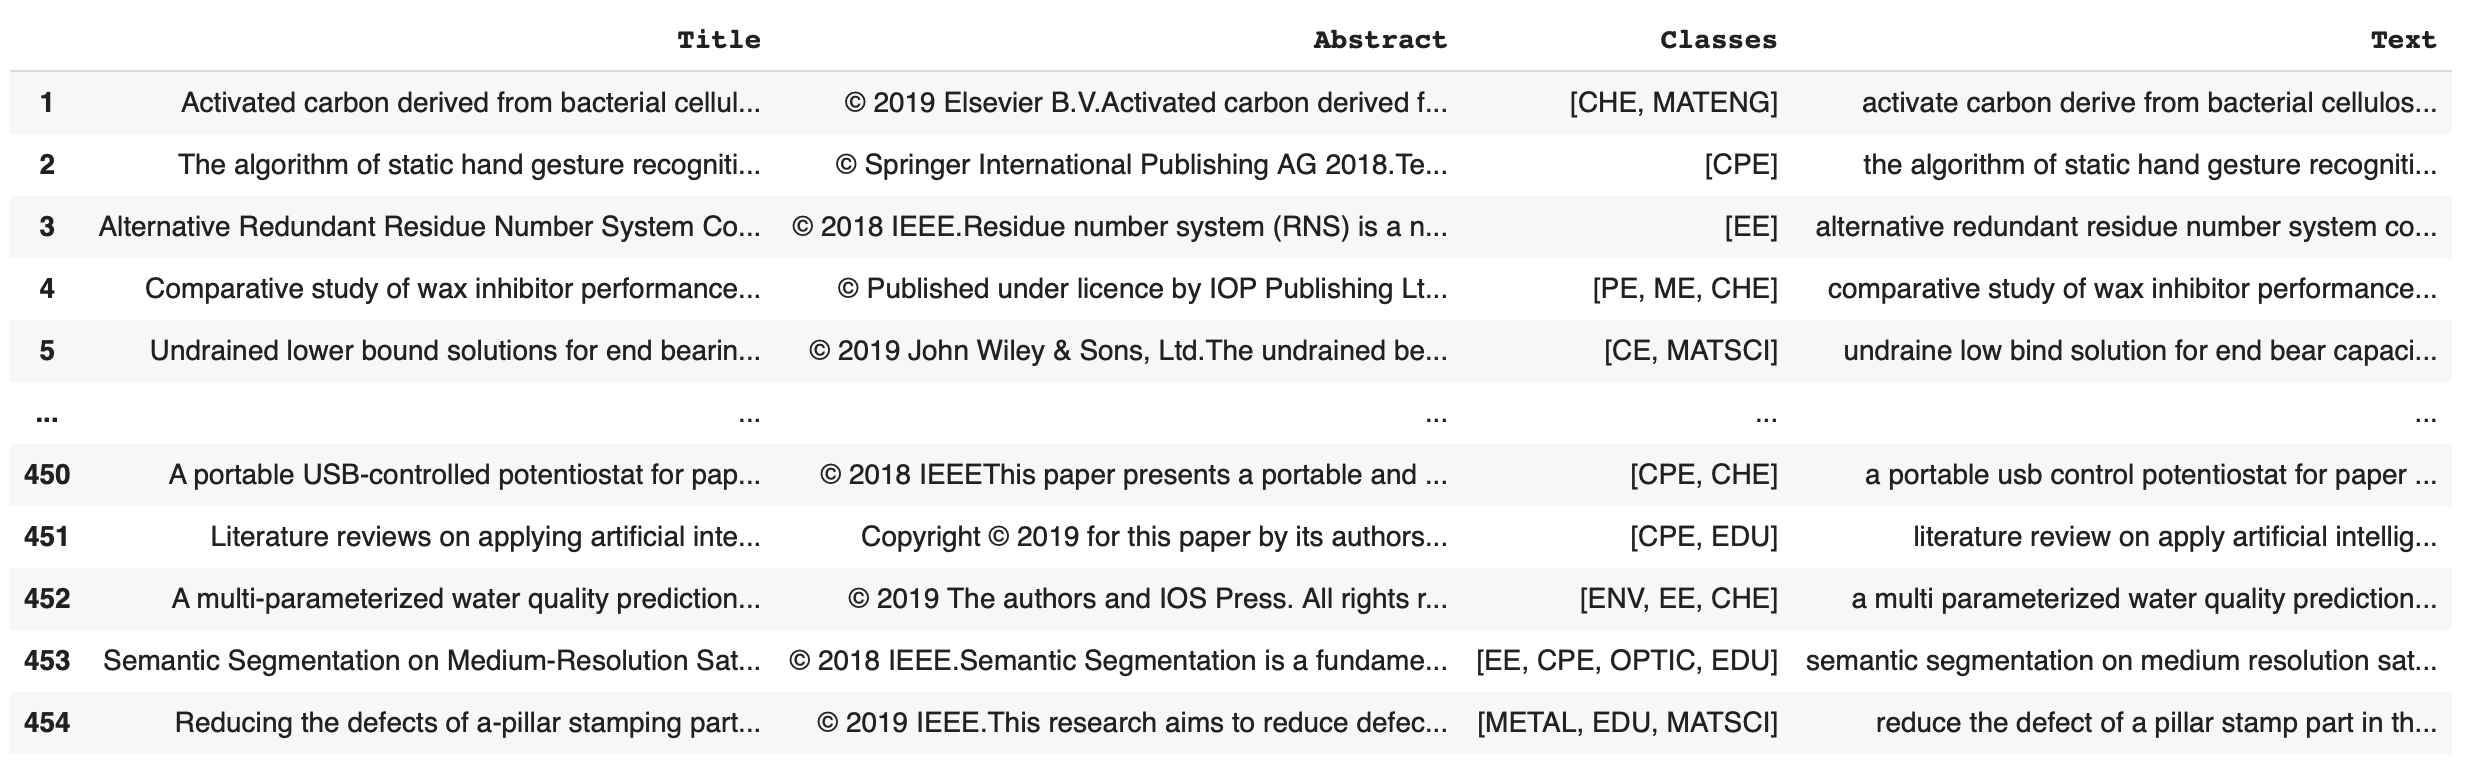
\includegraphics[width=\imgwidth]
    {images/dataframe_after_preprocessed.jpg}
    \caption{ข้อความที่อยู่ในคอลัมน์ Text เป็นข้อความที่ผ่านการ Preprocess แล้ว}
    \label{fig:dataframe_after_preprocessed}
\end{figure}
% Chapter 3: Model
\chapter{Model}

\section{Model Architecture}
ใช้ DistilBERT ซึ่งเป็น Pre-trained transformer model ด้วยเทคนิค distillation เป็นโมเดลที่มีขนาดเล็ก แต่ยังคงประสิทธิภาพส่วนใหญ่ไว้อยู่ \cite{victor2019distilbert} เนื่องจากข้อมูลมีจำนวนน้อย การ fine-tune โมเดลที่มีปริมาณ parameter น้อยจะสามารถทำได้ง่ายกว่า

สถาปัตยกรรมโมเดลประกอบด้วย pre-trained DistilBERT ตามด้วย fully connected layer ที่ใช้ sigmoid เป็น activation function ที่จะทำหน้าที่แปลง output embeddings เป็นคะแนนความน่าจะเป็นของแต่ละคลาสทั้ง 18 คลาส

\section{Training Configuration}
\begin{itemize}
    \item Optimizer: AdamW, learning rate 2e-5
    \item Loss function: BCEWithLogitsLoss, pos\_weight
    \item Batch size: 16
    \item Max length: 512
    \item Number of epochs: 30
\end{itemize}
\clearpage

\begin{figure}[ht]
    \centering
    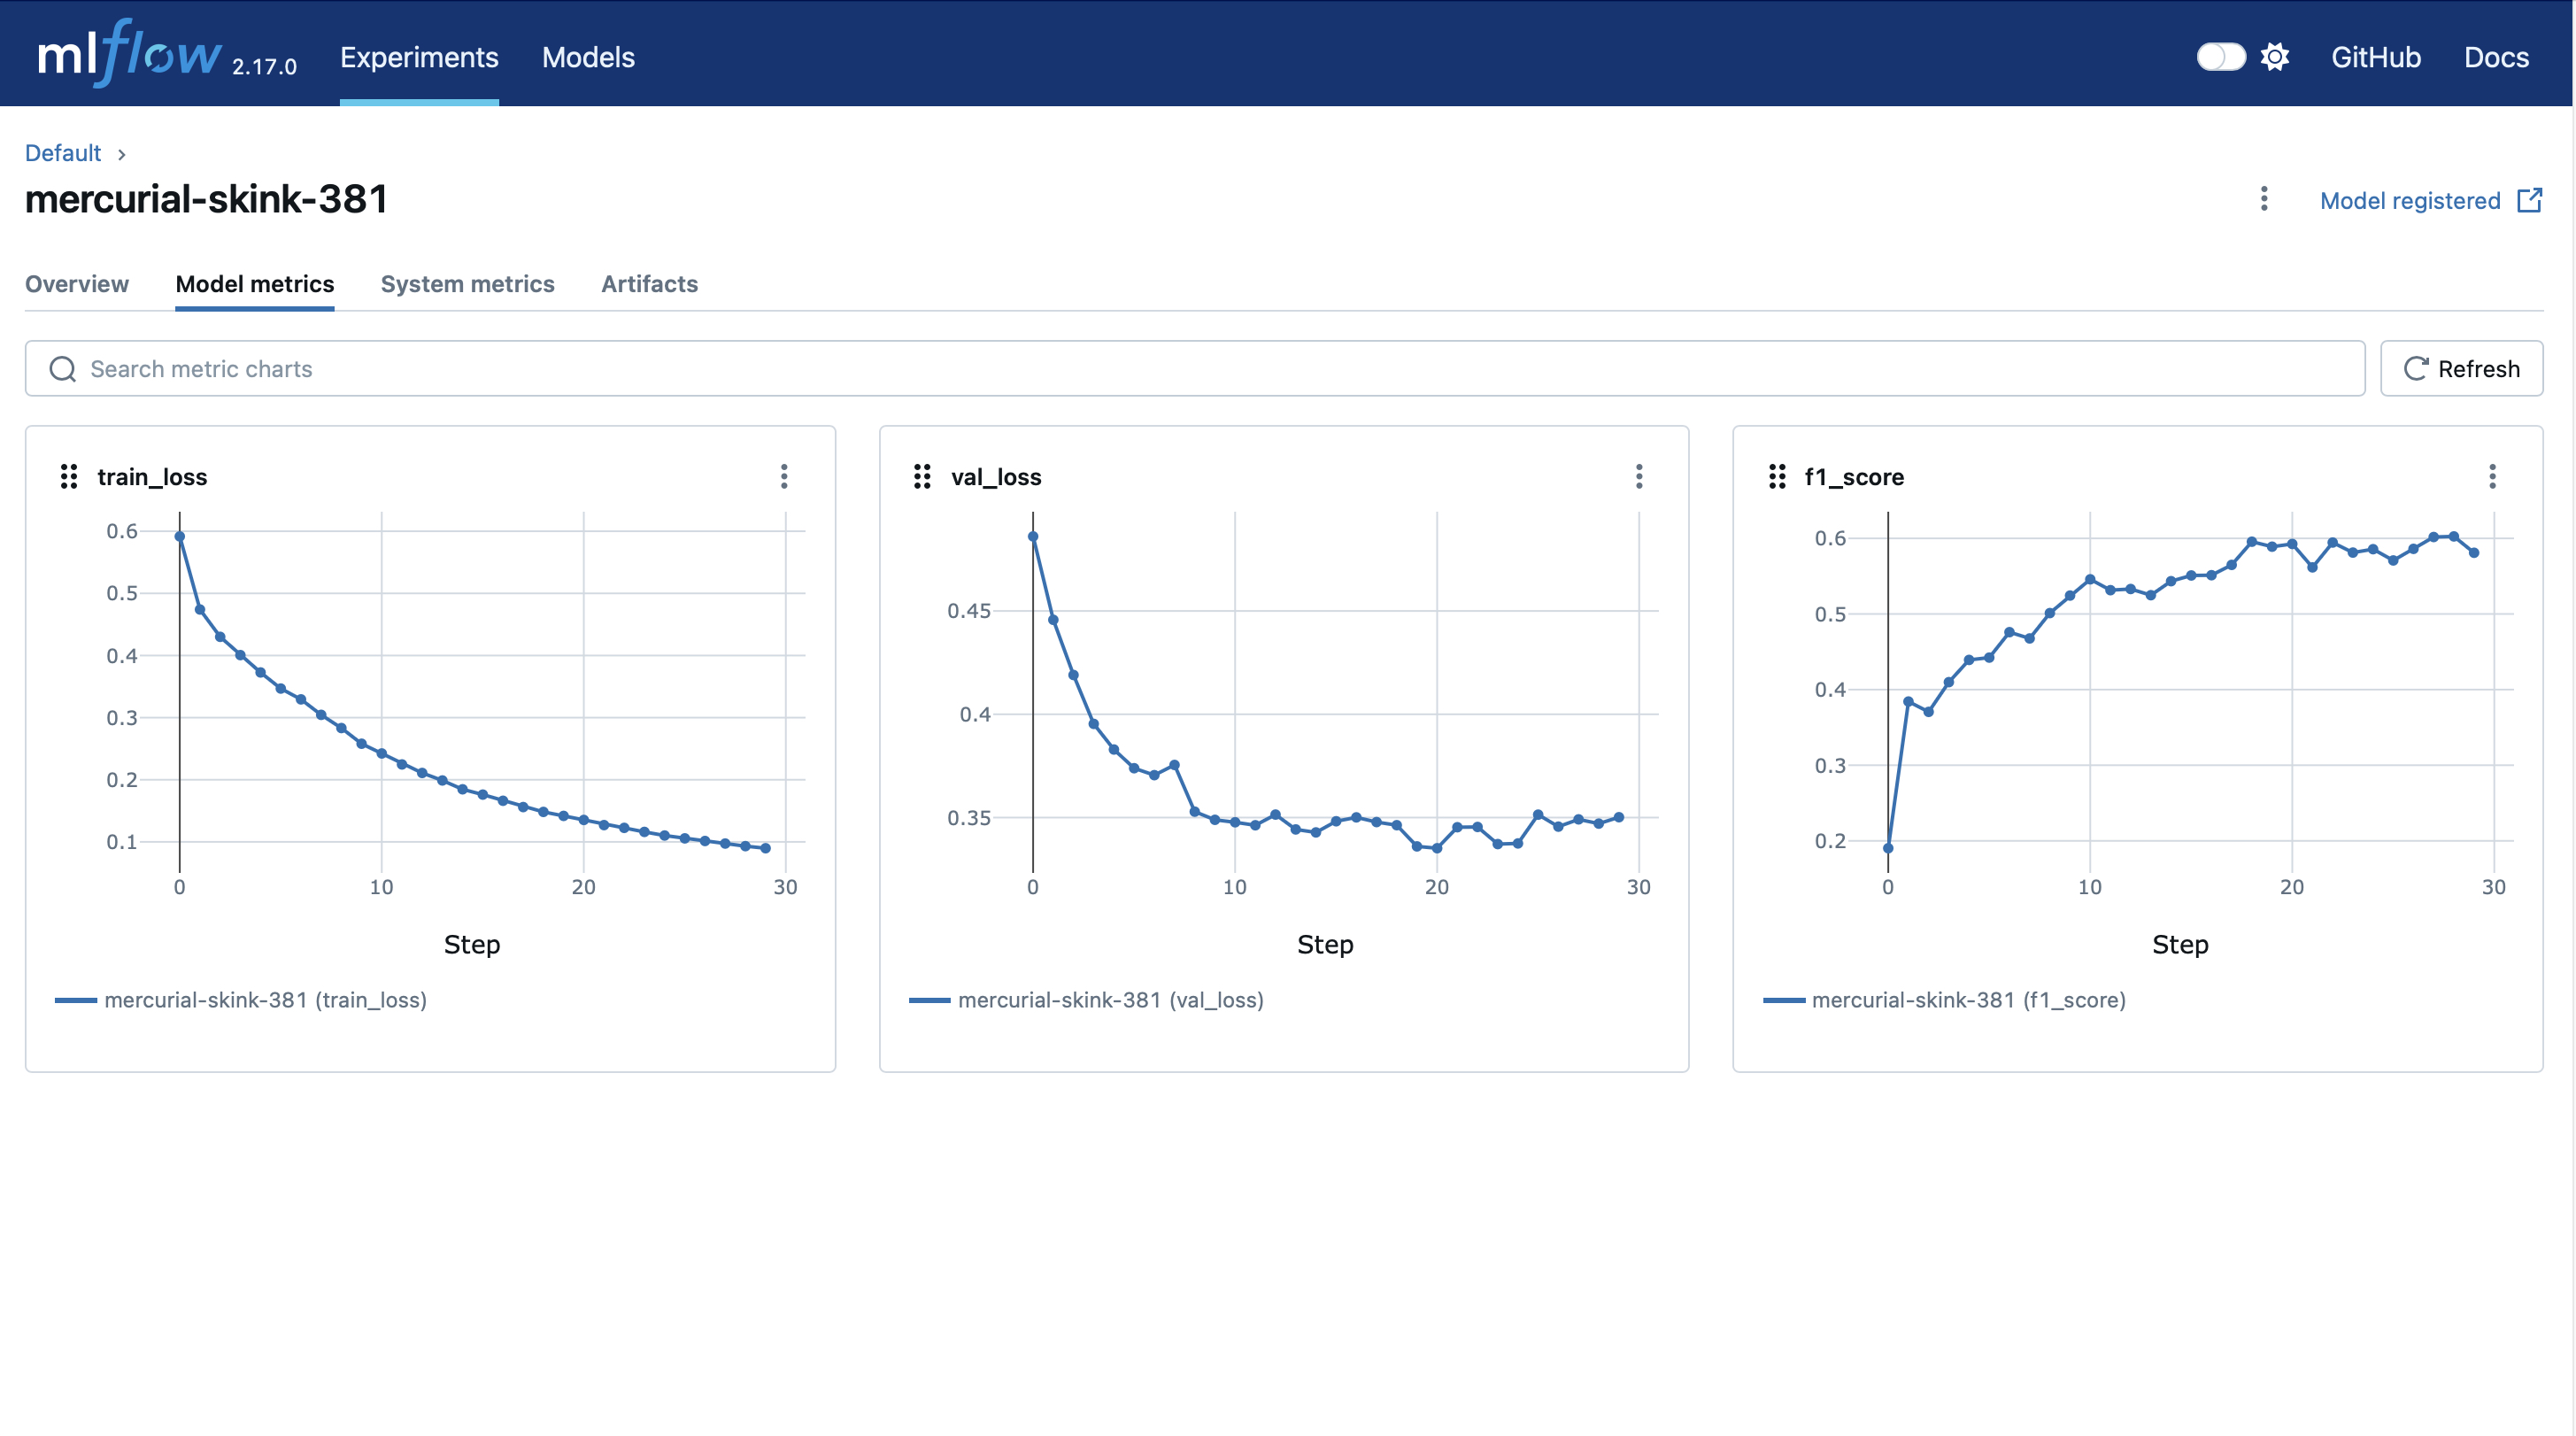
\includegraphics[width=\imgwidth]
    {images/model_training_graph.jpg}
    \caption{Model training graph}
    \label{fig:model_training_graph}
\end{figure}

\begin{figure}[ht]
    \centering
    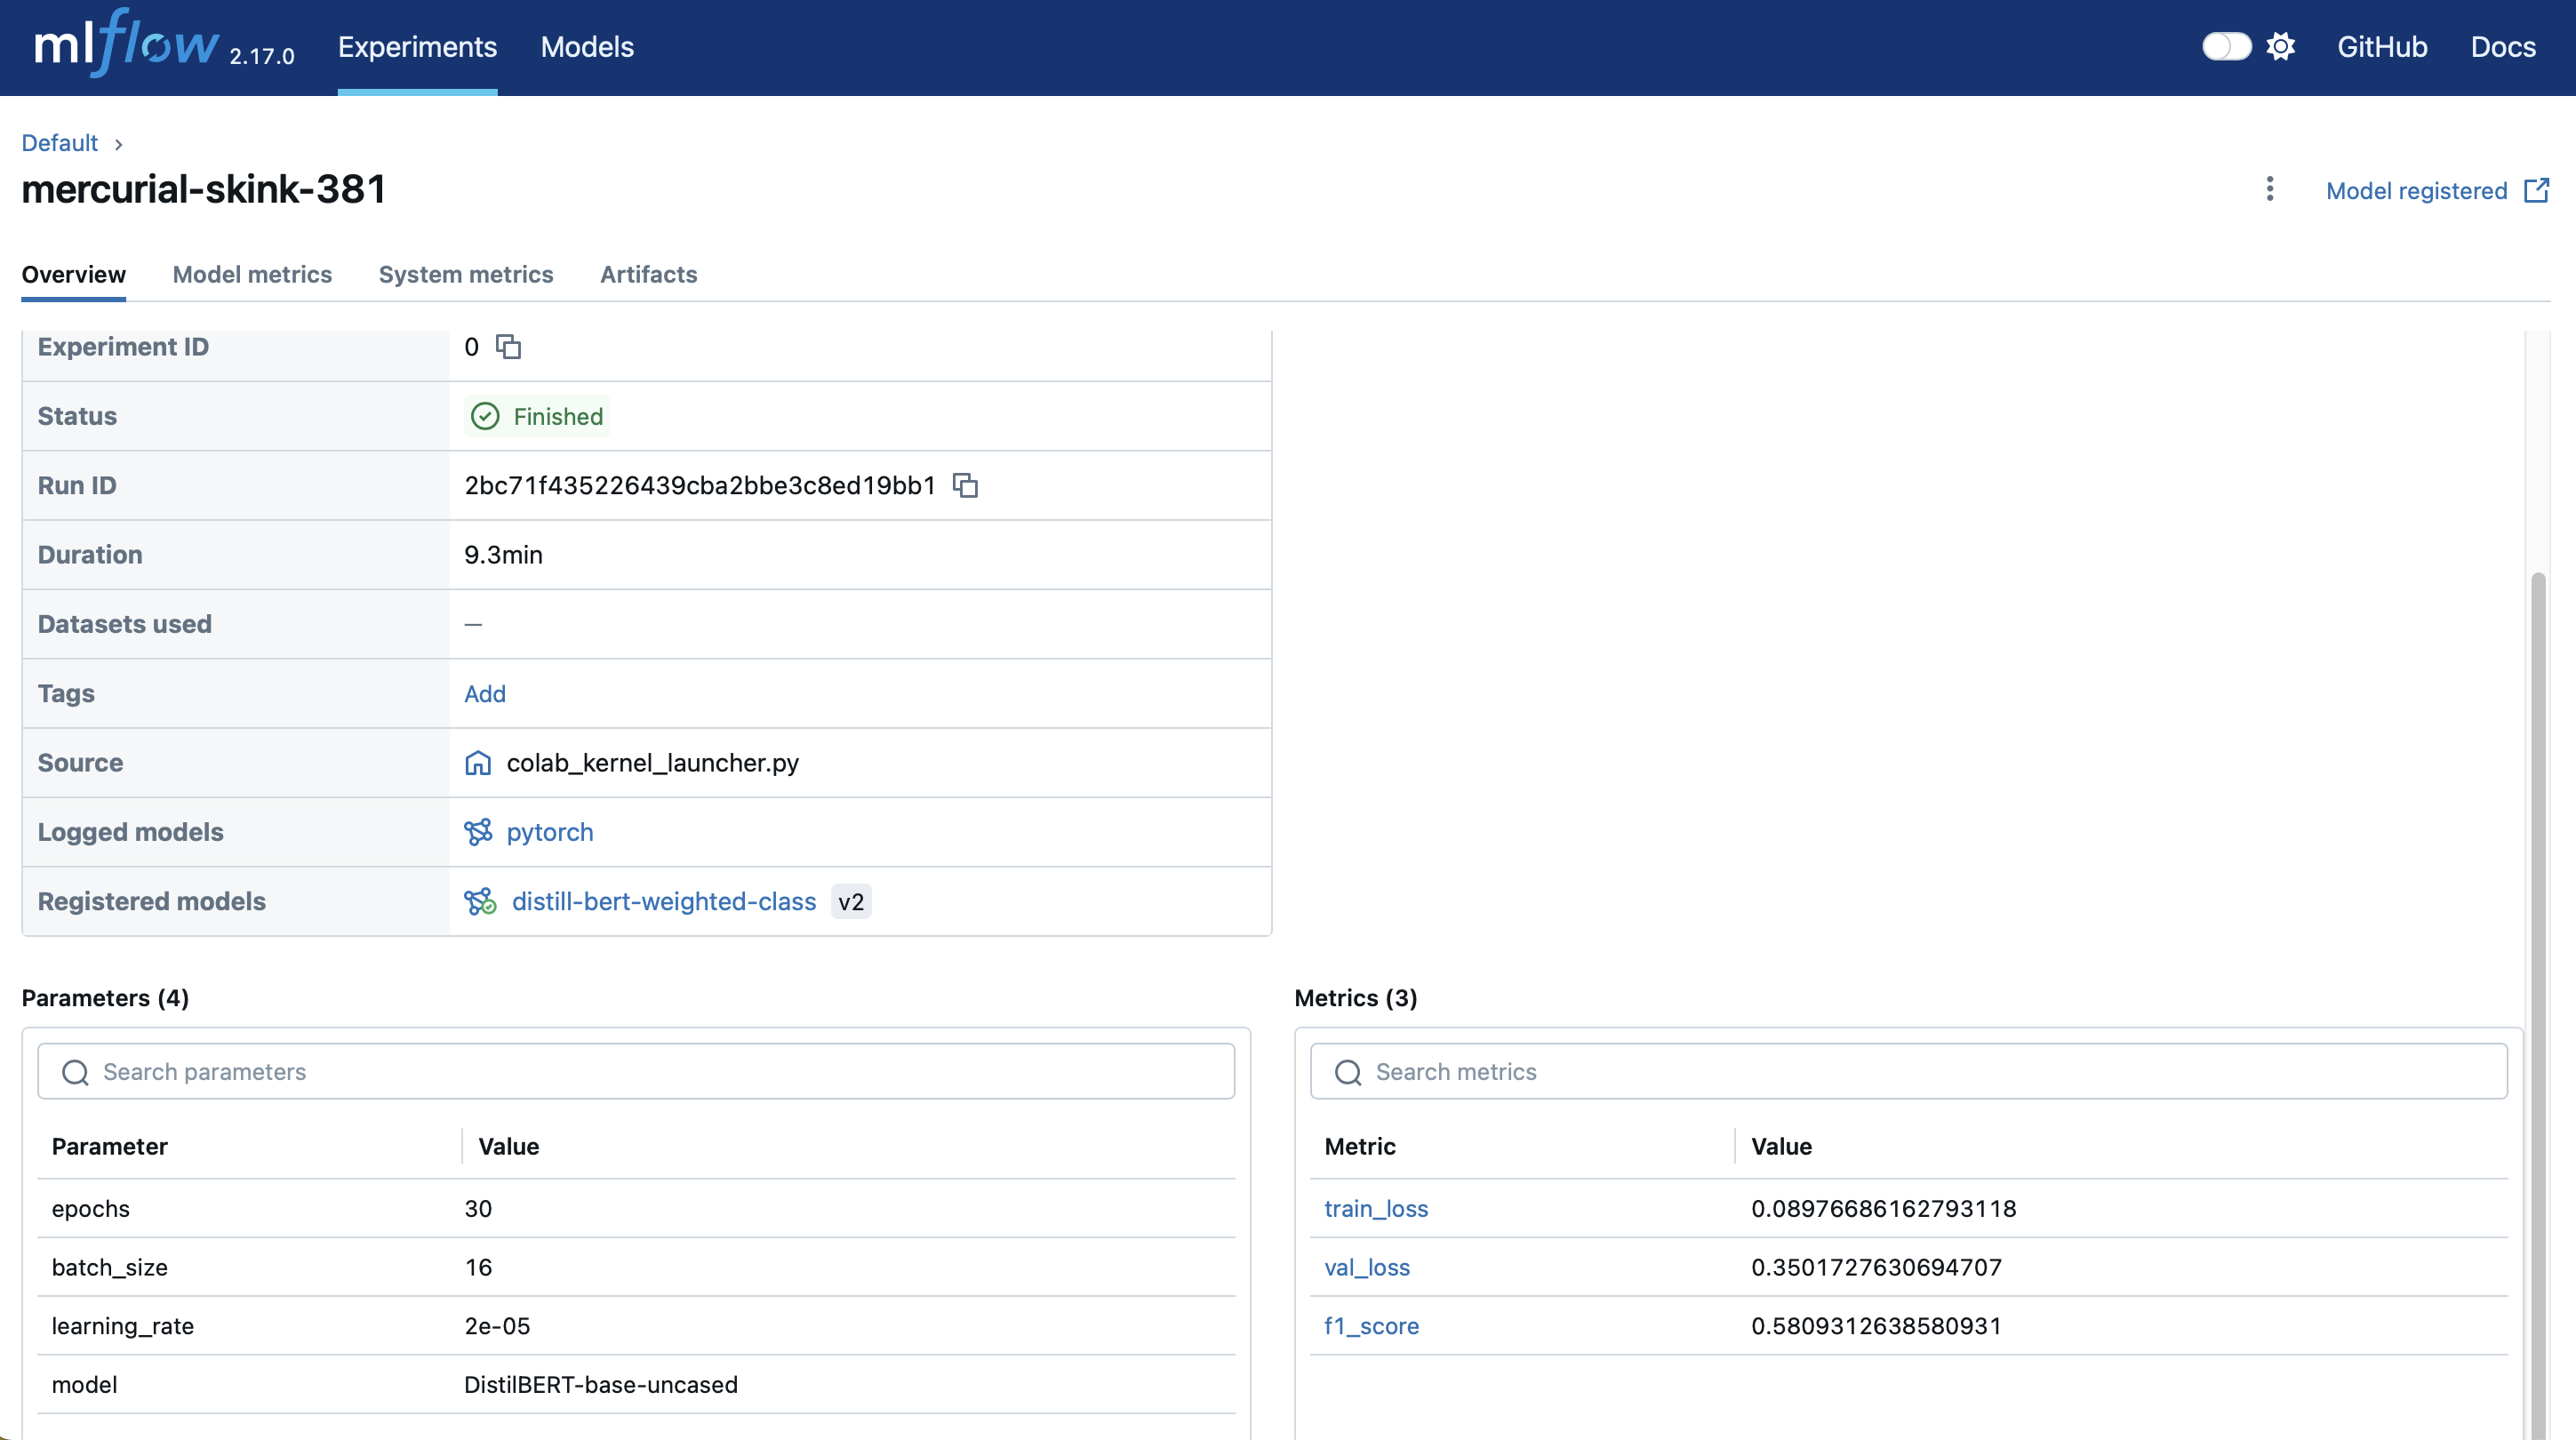
\includegraphics[width=\imgwidth]
    {images/model_metrics.jpg}
    \caption{Model metrics from MLflow}
    \label{fig:model_metrics.jpg}
\end{figure}

โมเดลมี F1 Validation อยู่ที่ 0.5809 และค่า val\_loss เริ่มลู่เข้าที่ Epoch 10
% Chapter 4: Results
\chapter{ผลลัพธ์}
\section{Kaggle Submission}
เมื่อนำโมเดลมาทำนาย Label ใน test.json
ได้ผลลัพธ์การ Submission ใน Kaggle ดังนี้
\begin{enumerate}
    \item Public Score 0.4268
    \item Private Score 0.4646
\end{enumerate}



\begin{figure}[ht]
    \centering
    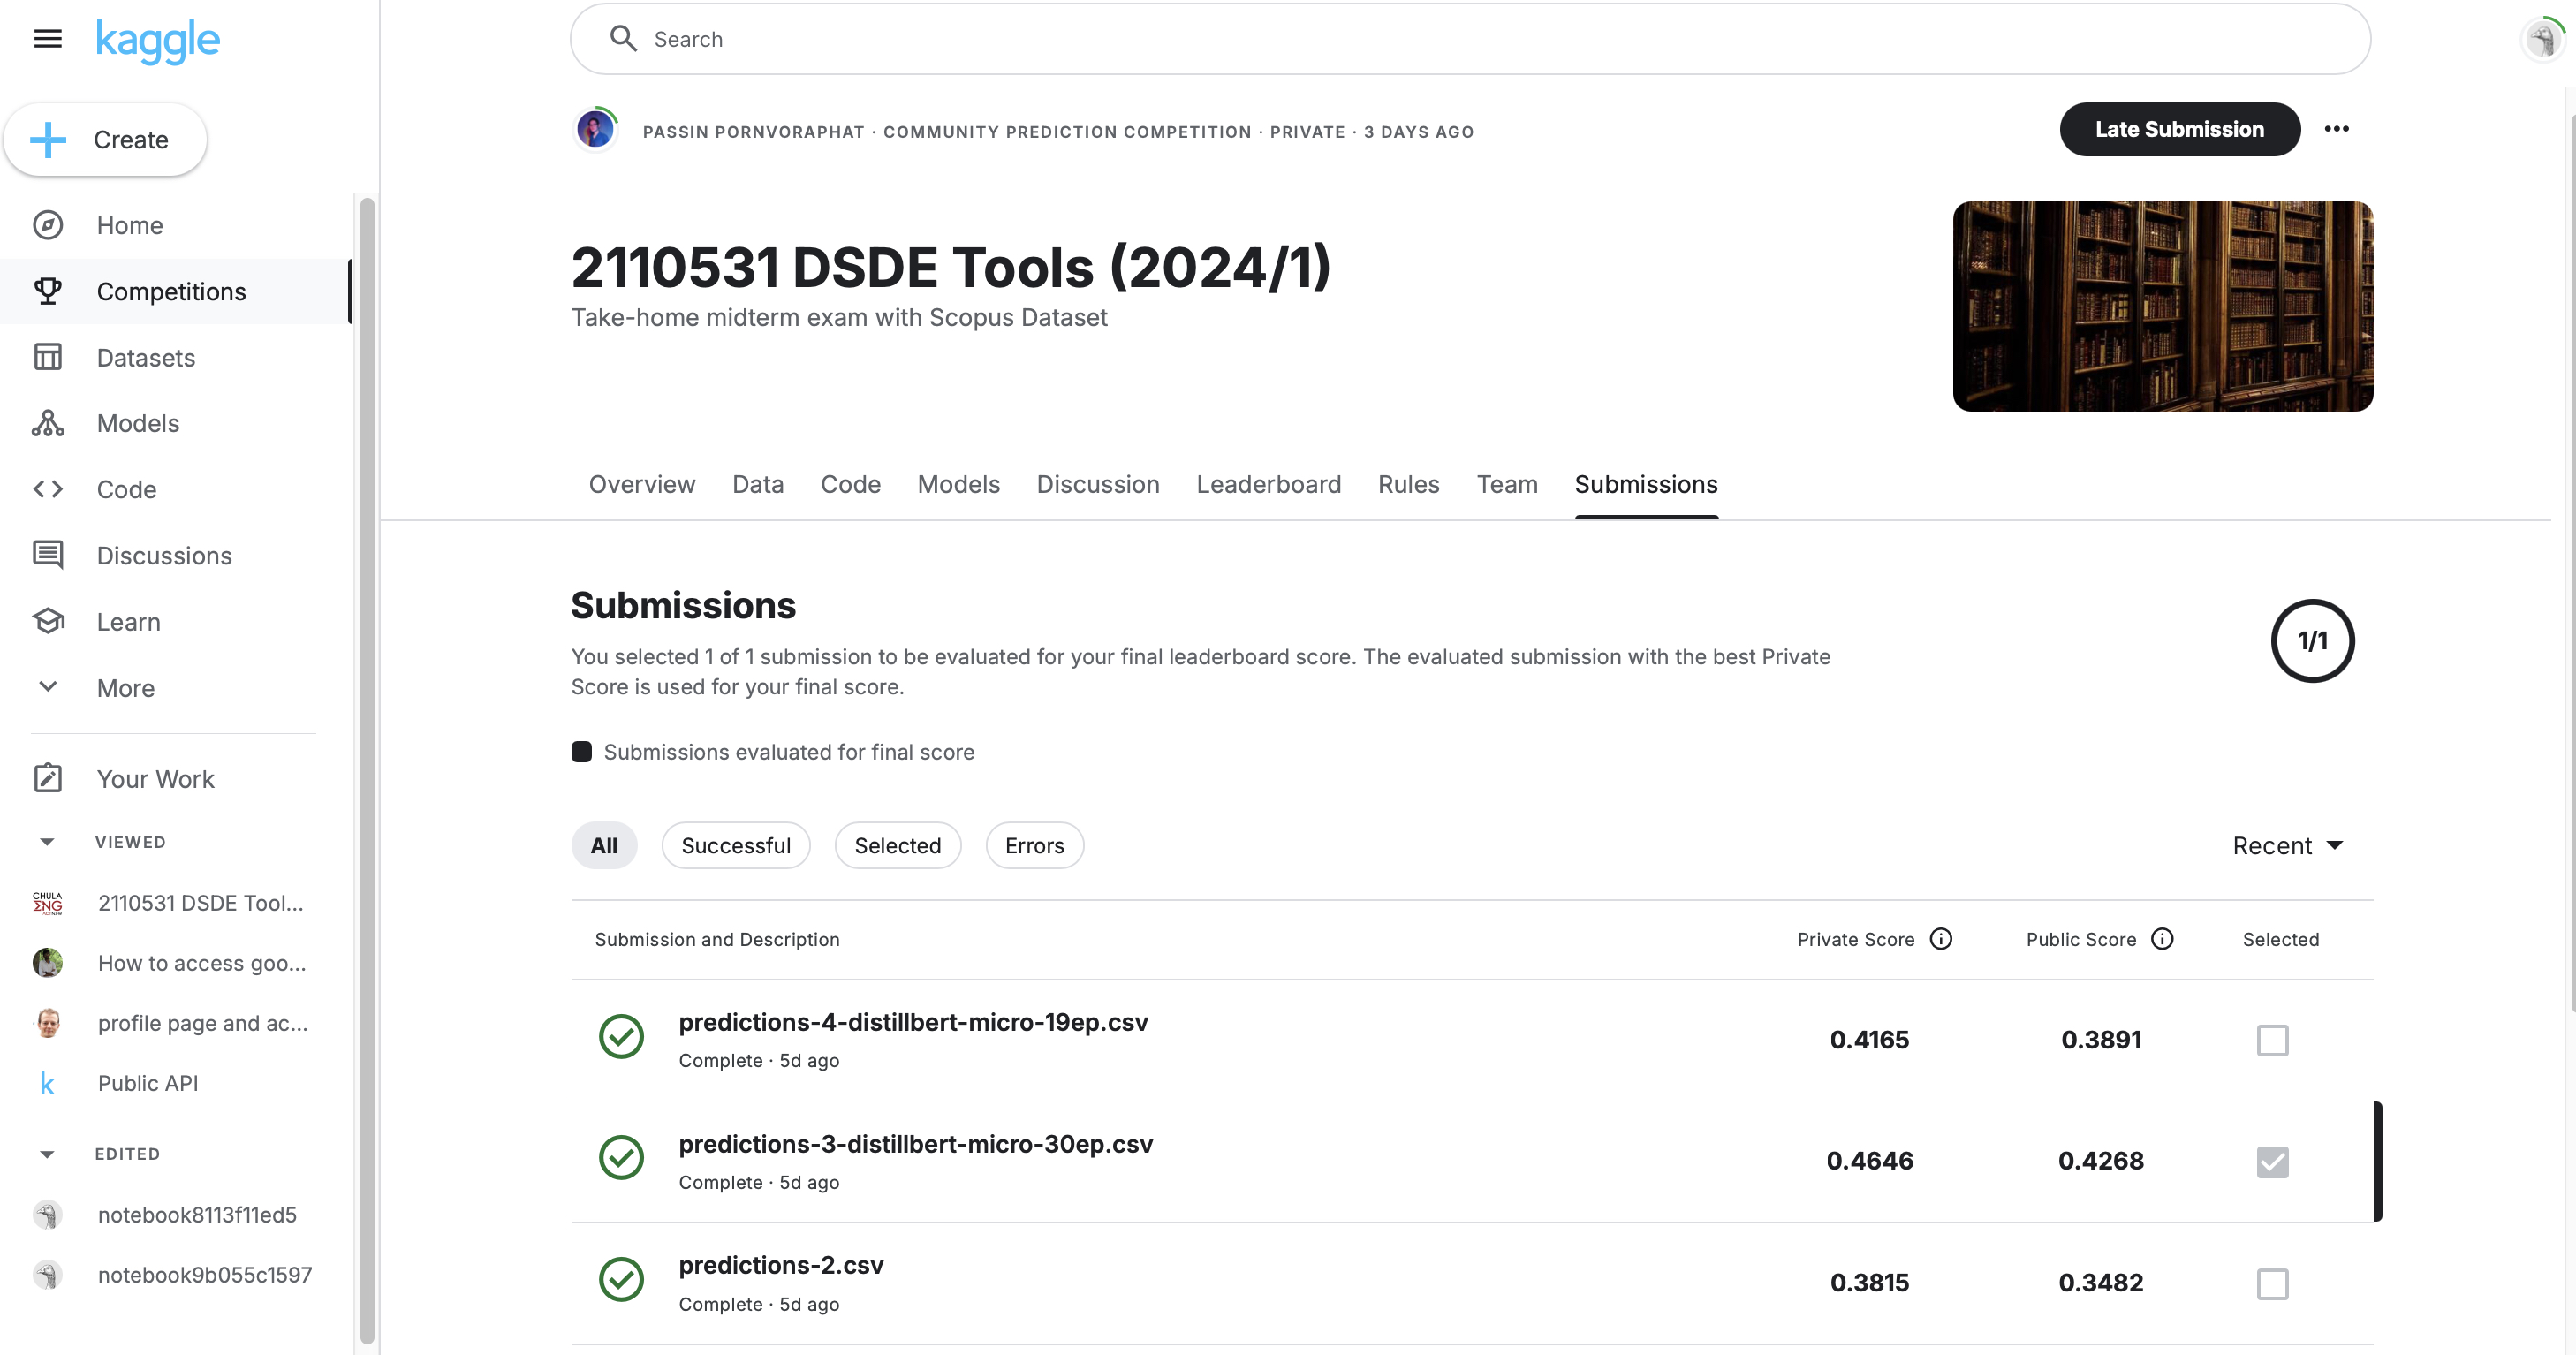
\includegraphics[width=\imgwidth]{images/kaggle_submission.jpg} 
    \caption{ผลการ Submission ใน Kaggle}
    \label{fig:kaggle_submission}
\end{figure}

\begin{figure}[ht]
    \centering
    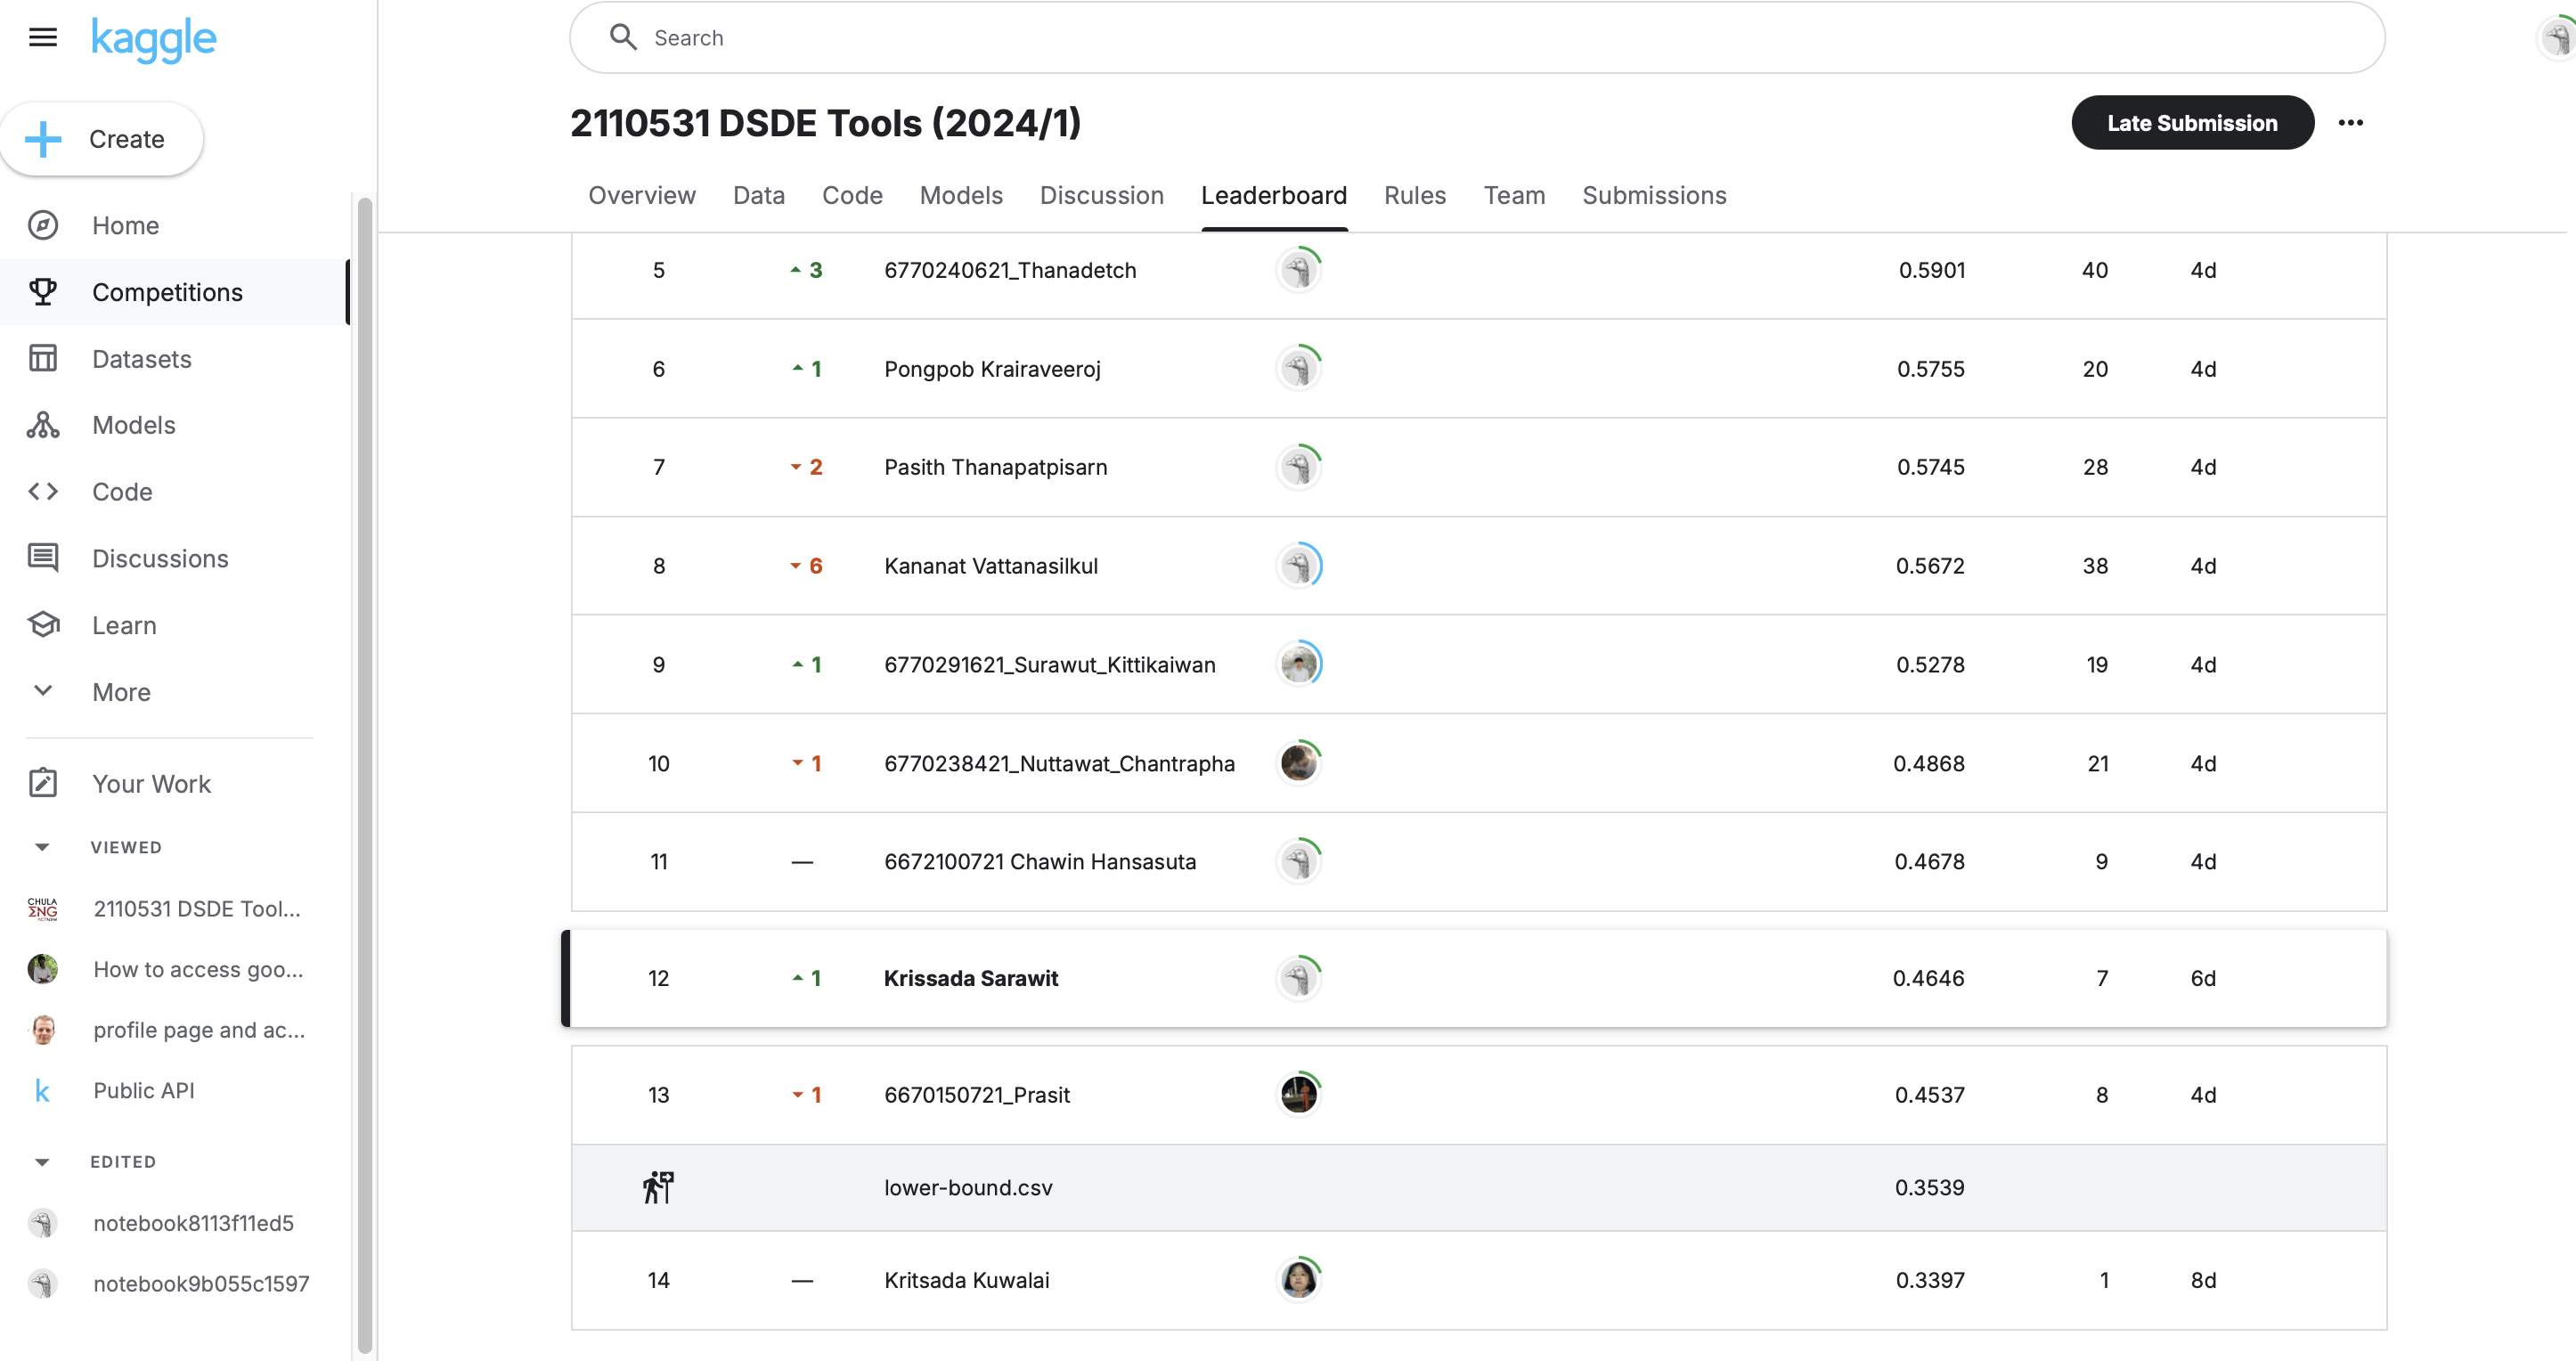
\includegraphics[width=\imgwidth]{images/kaggle_leaderboard.jpg} 
    \caption{Leaderboard ใน Kaggle}
    \label{fig:kaggle_leaderboard}
\end{figure}
\chapter{การอภิปราย}
\section{การเพิ่มประสิทธิภาพ}
จากการทดลองจะเห็นได้ว่า โมเดลไม่สามารถทำนาย Label ได้ดีนัก หากสามารถเพิ่มปริมาณข้อมูลที่ใช้ Fine-tune อาจเพิ่ม Performance ของโมเดลได้ โดยอาจทำได้โดย
\begin{enumerate}
    \item แปลภาษาข้อมูลเป็นภาษาที่สองแล้วแปลกลับมาเป็นภาษาเดิม (Back translation) เพื่อเพิ่มปริมาณข้อมูล
    \item การทำ Oversampling เพื่อลดปัญหา Imbalanced class
    \item การทำ Early stopping เพื่อป้องกันโมเดล Overfitting
    \item ใช้ Model ภาษาเฉพาะทางเช่น SciBERT ซึ่งเป็น BERT ที่ Train ด้วยข้อความในโดเมนวิทยาศาสตร์ ซึ่งจะทำให้โมเดลเข้าในข้อความในบริบทบทความทางวิศวกรรมได้ดีขึ้น
\end{enumerate}
\chapter{สรุปผล}

การทำนายหมวดหมู่ของเอกสารบทความทางวิศวกรรมโดยใช้โมเดลภาษาในงานนี้ โดยการปรับแต่งโมเดล (fine-tuning) DistilBERT เพื่อรองรับการจำแนกหมวดหมู่แบบหลายคลาส (multi-label classification) สำหรับหมวดหมู่ทางวิศวกรรมทั้ง 18 หมวดหมู่ โมเดลสามารถทำนายหมวดหมู่ของเอกสารความทางวิศวกรรมได้ถึงแม้ข้อมูลจะมีปริมาณน้อยและไม่สมดุล

อย่างไรก็ตามยังพบข้อจำกัดในการทำนายหมวดหมู่ ซึ่งการปรับปรุงโมเดลในอนาคตอาจพิจารณาการใช้เทคนิคการสุ่มตัวอย่างข้อมูลเพิ่มเติม (data augmentation) หรือการเพิ่มข้อมูลเพื่อแก้ไขปัญหาความไม่สมดุล หรือปรับโมเดลให้มีความซับซ้อนมากขึ้น ซึ่งอาจจะช่วยให้โมเดลสามารถทำนายได้อย่างแม่นยำมากขึ้น

% References 
\renewcommand{\bibname}{References}
\bibliographystyle{ieeetr}  
\bibliography{references} 

\end{document}